\documentclass[oneside,article]{memoir}
\usepackage{layouts}[2001/04/29]
\usepackage{xmpincl}	% Seems to be required to get the pdf to generate??

\makeglossary
\makeindex

\def\mychapterstyle{default}
\def\mypagestyle{headings}
\def\revision{}
%%% need more space for ToC page numbers
\setpnumwidth{2.55em}
\setrmarg{3.55em}

%%% need more space for ToC section numbers
\cftsetindents{part}{0em}{3em}
\cftsetindents{chapter}{0em}{3em}
\cftsetindents{section}{3em}{3em}
\cftsetindents{subsection}{4.5em}{3.9em}
\cftsetindents{subsubsection}{8.4em}{4.8em}
\cftsetindents{paragraph}{10.7em}{5.7em}
\cftsetindents{subparagraph}{12.7em}{6.7em}

%%% need more space for LoF numbers
\cftsetindents{figure}{0em}{3.0em}

%%% and do the same for the LoT
\cftsetindents{table}{0em}{3.0em}

%%% set up the page layout
\settrimmedsize{\stockheight}{\stockwidth}{*}	% Use entire page
\settrims{0pt}{0pt}

\setlrmarginsandblock{1.5in}{1.5in}{*}
\setulmarginsandblock{1.5in}{1.5in}{*}

\setmarginnotes{17pt}{51pt}{\onelineskip}
\setheadfoot{\onelineskip}{2\onelineskip}
\setheaderspaces{*}{2\onelineskip}{*}
\checkandfixthelayout

\usepackage{fancyvrb}			% Allow \verbatim et al. in footnotes
\usepackage{graphicx}			% To include graphics in pdf's (jpg, gif, png, etc)
\usepackage{booktabs}			% Better tables
\usepackage{tabulary}			% Support longer table cells
\usepackage[utf8]{inputenc}		% For UTF-8 support
\usepackage[T1]{fontenc}		% Use T1 font encoding for accented characters
\usepackage{xcolor}				% Allow for color (annotations)

%\geometry{landscape}			% Activate for rotated page geometry

%\usepackage[parfill]{parskip}	% Activate to begin paragraphs with an empty
								% line rather than an indent


\def\myauthor{Author}			% In case these were not included in metadata
\def\mytitle{Title}
\def\mykeywords{}
\def\mybibliostyle{plain}
\def\bibliocommand{}

\VerbatimFootnotes
\def\myauthor{Fletcher T. Penney}
\def\baseheaderlevel{2}
\def\mycopyright{2006-2009 Fletcher T. Penney. \\ This work is licensed under a Creative Commons License. \\ http://creativecommons.org/licenses/by-sa/3.0/}
\def\format{complete}
\def\mykeywords{MultiMarkdown, Markdown, XML, XHTML, XSLT, PDF,}
\def\latexxslt{article.xslt}
\def\rtfxslt{xhtml2rtf}
\def\mytitle{Sample MultiMarkdown Document}


%
%	PDF Stuff
%

%\ifpdf							% Removed for XeLaTeX compatibility
%  \pdfoutput=1					% Removed for XeLaTeX compatibility
  \usepackage[
  	plainpages=false,
  	pdfpagelabels,
  	pdftitle={\mytitle},
  	pagebackref,
  	pdfauthor={\myauthor},
  	pdfkeywords={\mykeywords}
  	]{hyperref}
  \usepackage{memhfixc}
%\fi							% Removed for XeLaTeX compatibility


%
% Title Information
%


\ifx\latexauthor\undefined
\else
	\def\myauthor{\latexauthor}
\fi

\ifx\subtitle\undefined
\else
	\addtodef{\mytitle}{}{ \\ \subtitle}
\fi

\ifx\affiliation\undefined
\else
	\addtodef{\myauthor}{}{ \\ \affiliation}
\fi

\ifx\address\undefined
\else
	\addtodef{\myauthor}{}{ \\ \address}
\fi

\ifx\phone\undefined
\else
	\addtodef{\myauthor}{}{ \\ \phone}
\fi

\ifx\email\undefined
\else
	\addtodef{\myauthor}{}{ \\ \email}
\fi

\ifx\web\undefined
	\else
		\addtodef{\myauthor}{}{ \\ \web}
\fi

\title{\mytitle}
\author{\myauthor}

\begin{document}

% Title
\mainmatter

\maketitle

% Copyright Info
\setlength{\parindent}{0pt}

\ifx\mycopyright\undefined
\else
	\textcopyright{} \mycopyright
\fi

\revision

\setlength{\parindent}{1em}

%
% Main Content
%


% Layout settings
\setlength{\parindent}{1em}

\chapter{Introduction}
\label{introduction}

As I add increasing numbers of features to MultiMarkdown, I decided it was
time to create a sample document to show them off. Many of the features are
demonstrated in the \href{http://fletcherpenney.net/mmd/users_guide/}{MultiMarkdown User's Guide}\footnote{\href{http://fletcherpenney.net/mmd/users_guide/}{http://fletcherpenney.net/mmd/users\_guide/}}, but some are not.


Additionally, it's easy for those features to get lost within all of the
technical documentation. This document is designed to {\itshape demonstrate}, not
describe, most of the features of MultiMarkdown.


\chapter{How to Use This Document}
\label{howtousethisdocument}

I suggest comparing the raw text source with the various final outputs (e.g.
PDF, XHTML, LaTeX, RTF) in order to see what can be accomplished. There will
be many similarities between output formats, but also a few differences.
Tables will end up in different places. Paragraphs won't break in the same
way. But these differences are superficial and are a result of trying to
optimize each format, without regard to identical output across formats (which
would be virtually impossible).


Remember, the main goal of Markdown$\backslash$MultiMarkdown is to allow you to create a
document in plain text, with minimal distraction from markup, that can be
transformed into a variety of high quality outputs. Or, to quote John Gruber:


\begin{quotation}
The overriding design goal for Markdown's formatting syntax is to make it as
readable as possible. The idea is that a Markdown-formatted document should be
publishable as-is, as plain text, without looking like it's been marked up
with tags or formatting instructions. While Markdown's syntax has been
influenced by several existing text-to-HTML filters, the single biggest source
of inspiration for Markdown's syntax is the format of plain text
email.~\cite{Gruber}
\end{quotation}

\chapter{Where Can I Get a Copy?}
\label{wherecanigetacopy}

You can download a zipfile containing multiple formats of this document:


\begin{itemize}


\item \href{http://fletcher.github.com/MultiMarkdown-Gallery}{MultiMarkdown-Gallery}\footnote{\href{http://fletcher.github.com/MultiMarkdown-Gallery}{http://fletcher.github.com/MultiMarkdown-Gallery}}
\end{itemize}

This file includes:


\begin{itemize}


\item The Scrivener source file

\item A plain text file in MultiMarkdown format

\item An XHTML file

\item A PDF

\item An RTF
\end{itemize}

All files were generated automatically from the MultiMarkdown source document.


\chapter{So, What Can This Document Demonstrate?}
\label{sowhatcanthisdocumentdemonstrate}

\section{Metadata}
\label{metadata}

First, take a look at the overall structure of the document. At the very
beginning is metadata, including a title, author, keywords, copyright
information, etc. Where possible, this metadata is put to appropriate use,
otherwise it is stored in a format designed to be easily read and minimally
distracting:


\begin{itemize}


\item In plain text and XHTML snippets\footnote{An XHTML snippet is my terminology for XHTML code that does not
include the \texttt{$<$html$>$}, \texttt{$<$head$>$}, and \texttt{$<$body$>$} tags. Most browsers will display
it properly, but it is not a complete XHTML document. Without a \texttt{$<$head$>$}
section there is nowhere to put metadata(e.g.\ there is no \texttt{$<$title$>$}).}, it is located at the top of the
document.




\item In a full XHTML document, is located in the \texttt{$<$head$>$} section, and the title
and CSS metadata, if present, are used appropriately.




\item In a PDF generated from my XSLT files, metadata is used to generate the
appropriate fields (title, author, keywords) in the PDF itself. Some PDF
readers will let you examine this data. Additionally, the title, subtitle,
author, and copyright are placed at the beginning of the document.




\item In a Scrivener document, you can put the metadata in the first File in the
Binder, but the preferred location is in the ``MultiMarkdown Settings{\ldots}''
pane (in the File Menu.)



\end{itemize}

There are a lot of standard metadata keys that can be used, or you can create
your own and use them as you see fit. Definitely a powerful feature.


\section{Structure}
\label{structure}

The next thing to look at is the overall structure of the document. You can
visualize a Markdown document as an outline, with different sections and
different levels within those sections. Based on your output format, these can
be used to generate headers, or sections, or even chapters. It's all based on
what tools you use to process the XHTML output.


Even within the XHTML document, however, you can make use of this structure to
allow easy navigation within the document. You can link directly to the
Introduction (\autoref{introduction}) (and to \autoref{introduction} when using LaTeX), for instance. And if you are creating a PDF, it will contain
a hierarchy of section names that you can use to allow easy navigation, if
your PDF reader supports this function.


\section{Footnotes}
\label{footnotes}

Footnotes are very easy to implement in MultiMarkdown, as described in the
MultiMarkdown Syntax Guide.\footnote{Here is the text of the footnote itself.}


\section{Tables}
\label{tables}

Tables can be quite useful for showing data in a meaningful way. As an
example, here is a table comparing MultiMarkdown vs. Crayons (\autoref{multimarkdownvs.crayons}).


\begin{table}[htbp]
\begin{minipage}{\linewidth}
\setlength{\tymax}{0.5\linewidth}
\centering
\small
\caption{MultiMarkdown vs. Crayons}
\label{multimarkdownvs.crayons}
\begin{tabulary}{\linewidth}{@{}lcc@{}} \\ \toprule 
Features&MultiMarkdown&Crayons \\\midrule
Melts in warm places&No&Yes \\
Mistakes can be easily fixed&Yes&No \\
Easy to copy documents for friends&Yes&No \\
Fun at parties&No\footnote{I guess it depends on what kind of parties you go to{\ldots}}&Why not? \\

		\bottomrule
	Minimum markup for maximum quality?&Yes&No \\

		\bottomrule
	\end{tabulary}
\end{minipage}
\end{table}

\section{Typographical conventions}
\label{typographicalconventions}

By incorporating John Gruber's \href{http://daringfireball.net/projects/smartypants/}{SmartyPants}\footnote{\href{http://daringfireball.net/projects/smartypants/}{http://daringfireball.net/projects/smartypants/}} program into your workflow, you
can generate more ``correct'' typographic punction in your XHTML pages, and in
your LaTeX source if you are generating PDF's---this includes en and em
dashes, and ellipses{\ldots}.


Very nice when you want to focus on writing, not grammar.


\section{Image Support}
\label{imagesupport}

If you choose to incorporate images in your documents, this can be easily done
as well. MultiMarkdown makes it easier to link to images and include various
attributes.


As an example, here is an image from my website---Nautilus Star (\autoref{nautilusstar}).  If you have a local copy of the image, you can include
the image in a pdf.


\begin{figure}
\begin{center}
\resizebox{307pt}{250pt}{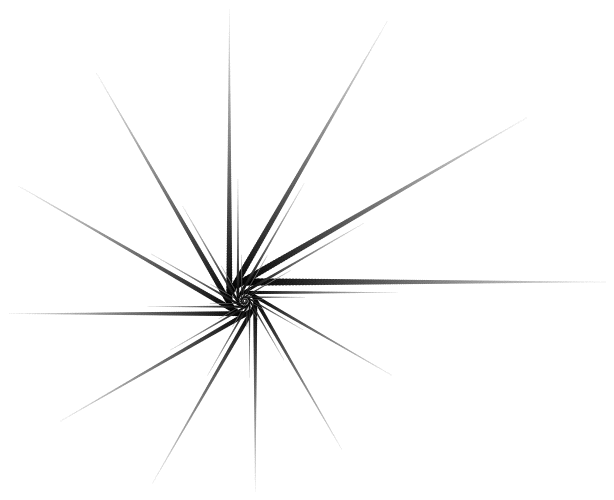
\includegraphics{Nautilus_Star.png}}
\end{center}
\caption{Nautilus Star}
	\label{nautilusstar}
\end{figure}



\section{Bibliography Support}
\label{bibliographysupport}

MultiMarkdown offers several mechanisms for managing bibliographies. It has
built-in support for basic citation and bibliography management and
formatting, or you can rely on external tools to handle this for you. There
aren't many citations in this document, but I think it gets the point
across.~\cite[p. 42]{fake}


\section{Glossary Support}
\label{glossarysupport}

MultiMarkdown has a special format for footnotes that should represent
glossary terms. This doesn't make much difference in XHTML (because there is
no such thing as a glossary in XHTML), but can be used to generate a glossary
within LaTeX documents.


For example, let's have an entry for \texttt{glossary}.\glossary{Glossary}{A section at the end {\ldots}} And what about
ampersands?\glossary(ampersand){\&}{A punctuation mark {\ldots}}


Since we want the ampersand entry to be sorted with the a's, and not with
symbols, we put in the optional sort key \texttt{ampersand} to control sorting.


\begin{adjustwidth}{2.5em}{2.5em}
\begin{verbatim}

[^glossary]: glossary: Glossary 
    A section at the end ...

[^amp]: glossary: & (ampersand)
    A punctuation mark ...

\end{verbatim}
\end{adjustwidth}

\section{Math Support}
\label{mathsupport}

It's pretty easy to include mathematical equations:


\begin{equation}
\label{eulersidentity}
{e}^{i\pi }+1=0
\end{equation}


\begin{equation}
\label{quadraticequationsolution}
{x}_{1,2}=\frac{-b\pm \sqrt{{b}^{2}-4ac}}{2a}
\end{equation}


You can also include formulas within a sentence, such as
${x}^{2}+{y}^{2}=1$.


\chapter{Now What?}
\label{nowwhat}

Get out there and try it. Let me know what you think. Let me know what doesn't
work. Let me know what you think is missing.


In other words, help me make it better!


You can get more information on my web site:


\begin{itemize}


\item \url{http://fletcherpenney.net/multimarkdown}
\end{itemize}

You can also:


\begin{itemize}


\item Email me: \\\href{mailto:owner@fletcherpenney.net}{owner@fletcherpenney.net}




\item Join the MultiMarkdown discussion list: \\\url{http://groups.google.com/group/multimarkdown}




\item Join the Markdown discussion list: \\\url{http://six.pairlist.net/mailman/listinfo/markdown-discuss}



\end{itemize}

\begin{thebibliography}{0}


\bibitem{Gruber}
John Gruber.  Daring Fireball: Markdown. [Cited January 2006]. Available from \url{http://daringfireball.net/projects/markdown/}.

\bibitem{fake}
John Doe. {\itshape A Totally Fake Book}.  Vanity Press, 2006.
		
\end{thebibliography}
		
%
% Back Matter
%

\backmatter
%\appendixpage

%	Bibliography
\bibliographystyle{\mybibliostyle}
\bibliocommand

%	Glossary
\printglossary


%	Index
\printindex

\end{document}
